
\section{Background}

\subsection{Convolution Operations}
In this paper, we use $I$, $F$ and $O$ to denote an input, a filter and an output tensor respectively. Each tensor is indexed according to
its batch size ($N$), channel ($C$), height ($H$) and width ($W$). For example, $I_N$, $I_C$, $I_H$ and $I_W$ represent the batch size,
number of channels, width and height of an input, $I$.

At the convolutional stage, the computational kernel takes as input a batch ($I_N$) of 2D feature maps of size $I_C \times I_H \times I_W$
and a bank ($F_N$) of  2D multi-channel filters of size $F_C \times F_H \times F_W$ ($F_C = I_C$). The computation produces a batch of
$O_N$ (where $O_N=I_N$) 2D multi-channel output feature maps of size $O_C \times O_H \times O_W$ ($O_C=F_N$). To compute one output feature
map, all filters are used to convolve with the same input feature map. Specifically, each filter slides over the input feature map to
perform an elementwise multiplication with the part of input where it is currently located and then sums up the results across all
channels.

\begin{figure}
\centering
  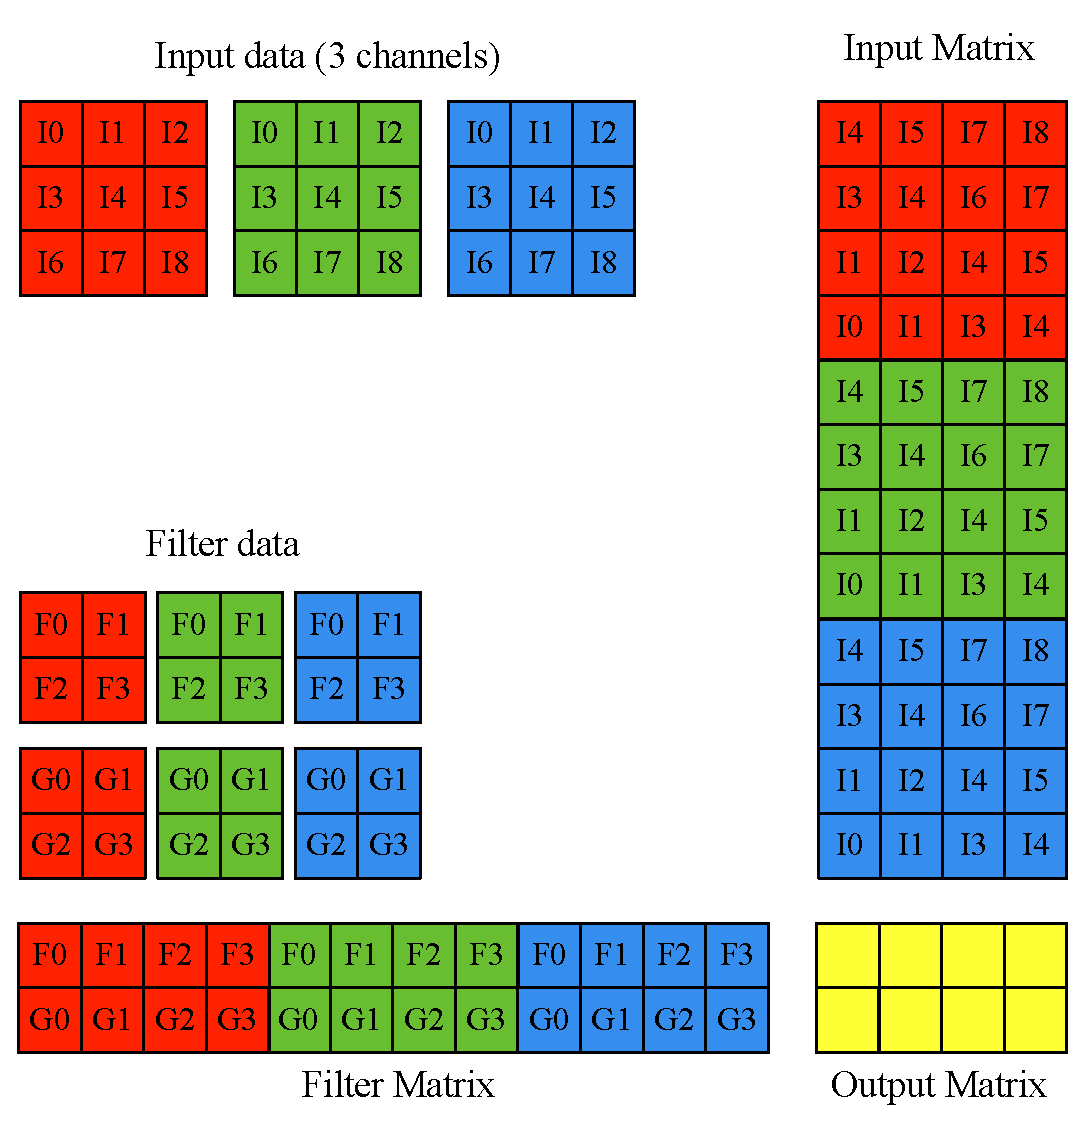
\includegraphics[width=0.75\columnwidth,height=6cm]{./figure/convlowering.eps}
  \caption{An example (reproduced from \cite{ChetlurWVCTCS14}) of converting a simple convolution into matrix multiplications. Here, two filters are used to convolve with a 3-channel input.}
  \label{fig:convlowering}
\end{figure}

Several algorithms, including FFT-based and Winograd-based convolutions, have been proposed to optimize the convolution operation. All
these approaches require to transform 4D tensors into the desired matrix, thus incurring high memory overhead. For example, Figure
\ref{fig:convlowering} illustrates how to translate a simple convolution into matrix multiplications. This process introduces numerous
duplicate elements. The redundant elements increase the memory footprint which can outweigh the performance gain by reducing the
computation complexity.

\subsection{Overview of Our Approach}
\begin{figure}[t!]
\centering
  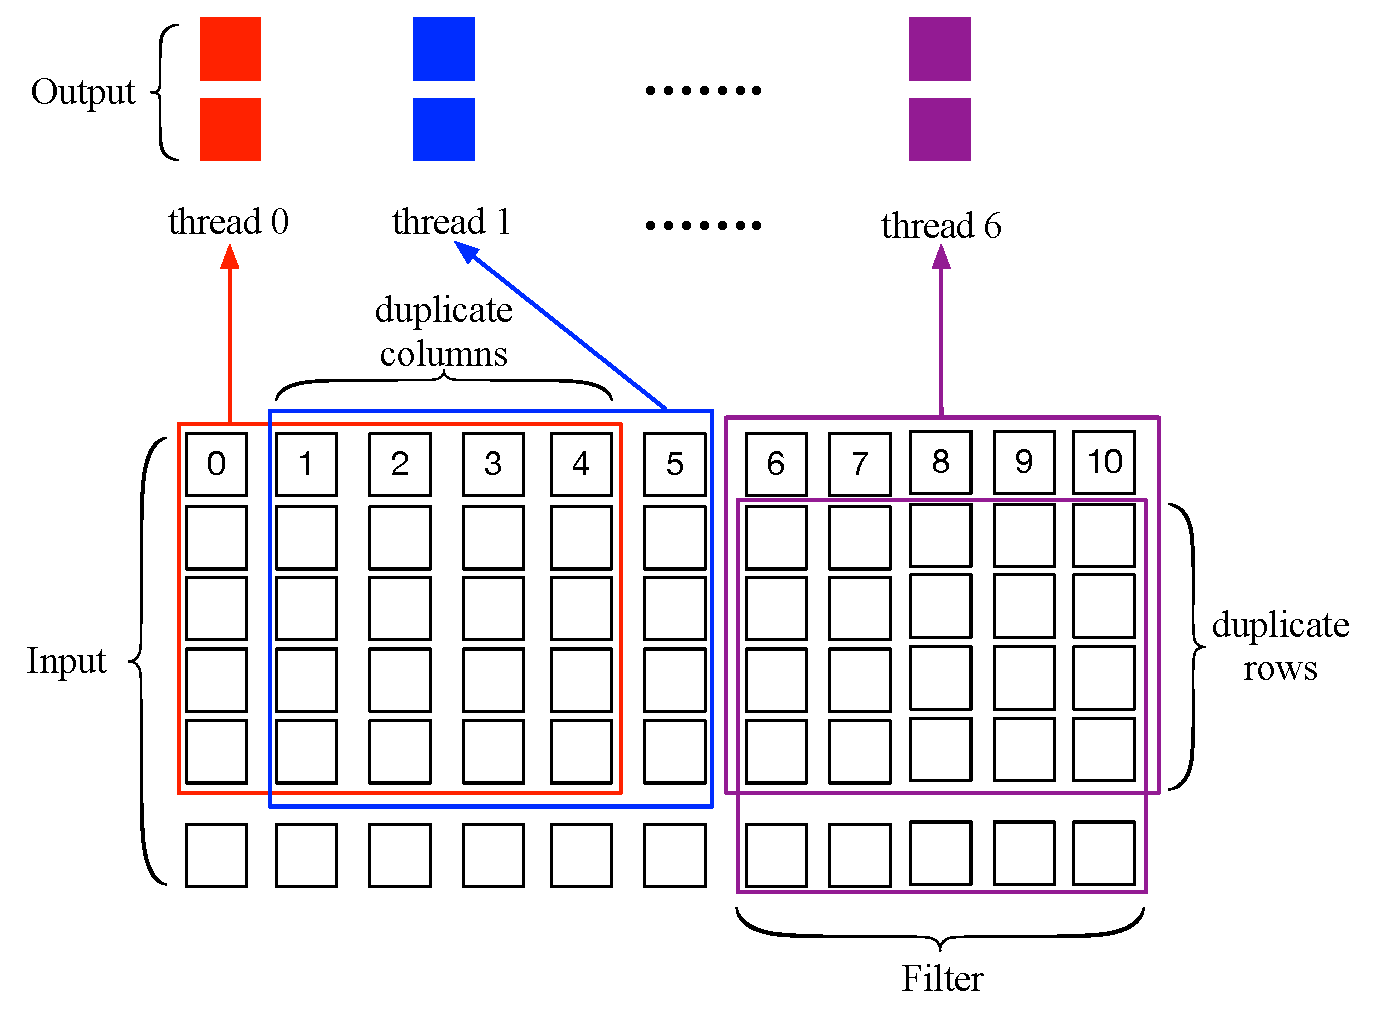
\includegraphics[width=\columnwidth,height=6cm]{./figure/twostrategies.eps}
  \caption{Example of performing 2D convolution using a GPU. Here, the filter size is $5 \times 5$, the input image size is $6 \times 11$
  and the output size is $2 \times 7$. Each thread calculates one column of the output. Assume threads 0 and 1 load the required regions from input
  image with four duplicate columns, and thread 6 loads two overlapped regions from input image and generates four duplicate rows. Numbers in
  the square denote the index of input elements.}
  \label{fig:twostrategies}
\end{figure}
As a motivation example, consider Figure \ref{fig:twostrategies} that shows a simple 2D convolution executing on a GPU. Here, we slide a $5
\times 5$ filter over a $6 \times 11$ image to produce a $2 \times 7$ output. In this example, each parallel GPU thread calculates one
column of the output. For example, threads 0 and 1 could execute code to slide the filter along the width dimension. Both threads load two
overlapped regions from the input image, thereby generating four duplicate columns. Assume thread 6 demonstrates the process of sliding the
filter along the height dimension. It loads two overlapped regions and generates four duplicate rows.

Our approach can eliminate redundant elements on the column and the width dimensions to reduce the number of memory accesses.  In the
proposed column reuse algorithm, we let each thread load the required first and last columns and retrieve the remaining from other threads
through shuffle instructions. The difference in the usage of shuffle instructions between our algorithms and the previous study
\cite{vasilache2014fast} is discussed in Section \ref{sec:strategies}. In the proposed row reuse algorithm, we let each thread load
overlapped rows only once and multiply each row with multiple rows of a filter to calculate multiple output elements. A major performance
issue encountered in our implementation is that the thread local arrays with dynamic indexing are placed in the local memory, which
possesses the same access latency as the global memory. To solve this problem, we use pack and unpack operations to transform dynamic
indexing into static indexing.
